% !TEX root = ../thesis-index.tex


\chapter{Batch Normalization Orthogonalizes Representations}\label{ch:bn_ortho}

Batch Normalization (BN)~\citep{ioffe2015batch} enhances training across a wide range of deep network architectures and experimental setups~\citep{he2016deep,huang2017densely,silver2017mastering}. The practical success of BN has inspired research into the underlying mechanism of BN~\citep{santurkar2018does,karakida2019normalization,arora2018theoretical,bjorck2018understanding}.
BN influences first-order optimization methods by avoiding the rank collapse in deep representation \citep{daneshmand2020batch},  direction-length decoupling of optimization \citep{kohler2018exponential}, influencing the convergence of the steepest descent  \citep{arora2018theoretical,bjorck2018understanding}, and smoothing the optimization objective function \citep{santurkar2018does,karakida2019normalization}. However, the benefits of BN go beyond its critical role in optimization. For example, \cite{frankle2020training} shows that BN networks with random weights also achieve surprisingly high performance after only minor adjustments of their weights. This striking result motivates us to study the representational power of random networks with BN.  


We study hidden representations across layers of a laboratory random BN with linear activations. Consider a batch of samples passing through consecutive BN and linear layers with Gaussian weights. The representations of these samples are perturbed by each random linear transformation, followed by a non-linear BN. At first glance, the deep representations appear unpredictable after many stochastic and non-linear transformations. Yet, we show that these transformations orthogonalize the representations. To prove this statement, we introduce the notion of  ``orthogonality gap'', defined in Section \ref{ortho:sec:orthogonality}, to quantify the deviation of representations from a perfectly orthogonal representation. Then, we prove that the orthogonality gap decays exponentially with the network depth and stabilizes around a term inversely related to the network width. More precisely, we prove 
\begin{align} \nonumber
     \E\Bigg[ \text{orthogonality gap} \Bigg] = \bigo\left( \left(1-\alpha\right)^{\text{depth}}+ \frac{\text{batchsize}}{\alpha\sqrt{\text{width}}}\right)
\end{align}
holds for $\alpha>0$ that is an absolute constant under a mild assumption. In probability theoretic terms, we prove stochastic stability of the Markov chain of hidden representations \citep{kushner1967stochastic,kushner2003stochastic,khasminskii2011stochastic}. The orthogonality of deep representations allows us to prove that the distribution of the representations after linear layers contracts to a Wasserstein-2 ball around isotropic Gaussian distribution as the network depth grows. Moreover, the radius of the ball is inversely proportional to the network width. Omitting details, we prove the following bound holds:
\begin{align} \nonumber
    \text{Wasserstein}_2(\text{representations},\text{Gaussian})^2= \bigo\left( \left(1-\alpha\right)^{\text{depth}}\left(\text{batchsize}\right)+ \frac{ (\text{batchsize})^2}{\alpha\sqrt{\text{width}}}\right).
\end{align}
The above equation shows how depth,  width, and batch size, interact with the Gaussian approximation of the representations. Since the established rate is exponential with depth, the distribution of the representations stays in a Wasserstein ball around isotropic Gaussian distribution after a few layers. Thus, BN not only stabilizes the distribution of the representations, which is its main promise~\citep{ioffe2015batch}, but also enforces Gaussian isotropic distribution in deep layers. 

There is growing interest in bridging the gap between neural networks, as the most successful parametric methods for learning, and Gaussian processes and kernel methods, as well-understood classical models for learning \citep{jacot2018neural,matthews2018gaussian,lee2017deep,bietti2019inductive,huang2014kernel}. This link is inspired by studying random neural networks in the asymptotic regime of infinite width. The seminal work by \cite{neal2012bayesian} sparks that a single-layer network resembles a Gaussian process as its width goes to infinity. However, increasing the depth may significantly shift the distribution of the representations away from Gaussian \citep{ioffe2015batch}. This distributional shift breaks the link between Gaussian processes and deep neural networks. To ensure Gaussian representations,  \cite{matthews2018gaussian} suggests increasing the width of the network proportional to the network depth. Here, we show that BN ensures Gaussian representations even for deep networks with \textit{finite} width. This result bridges the link between deep neural networks and Gaussian processes in the regime of finite width. Many studies rely on deep Gaussian representations in an infinite width setting \citep{yang2018a,schoenholz2016deep,pennington2018emergence,klambauer2017self,de2018random}. Our non-asymptotic Gaussian approximation can be incorporated into their analysis to extend these results to the regime of finite width.

Since training starts from random networks,  representations in these networks directly influence training. Hence, recent  theoretical studies has investigated the interplay between initial hidden representations and training~\citep{daneshmand2020batch,bjorck2018understanding,frankle2020training,schoenholz2016deep,saxe2013exact,bahri2020statistical}.
In particular, it is known that hidden representations in random networks \emph{without BN} become correlated as the network grows in depth, thereby drastically slowing training~\citep{daneshmand2020batch,he2016deep,bjorck2018understanding,saxe2013exact}. 
On the contrary,  we prove that deep representations in networks \emph{with BN} are almost orthogonal.
We experimentally validate that initial orthogonal representations can save training time that would otherwise be needed to orthogonalize them. By proposing a novel initialization scheme, we ensure the orthogonality of hidden representations. Such an initialization effectively avoids the training slowdown with depth for vanilla networks, with no need for BN.  This observation further motivates studying the inner workings of BN to replace or improve it for deep learning. \\
Theoretically, we made the following contributions:
\begin{enumerate}
    \item  For MLPs with batch normalization, linear activation, and Gaussian weights, we prove that representations across layers become increasingly orthogonal up to a constant inversely proportional to the network width. 
    \item Leveraging the orthogonality, we prove that the distribution of the representations contracts to a Wasserstein ball around a Gaussian distribution as the depth grows. Up to the best of our knowledge,  this is the first \textit{non-asymptotic} Gaussian approximation for deep neural networks with finite width.
\end{enumerate}
Experimentally, we made the following contribution\footnote{Implementations are available at \href{https://github.com/hadidaneshmand/batchnorm21.git}{https://github.com/hadidaneshmand/batchnorm21.git}}: 
\begin{enumerate}[resume]
    \item  Inspired by our theoretical understanding, we propose a novel weight initialization for standard neural networks that ensure orthogonal representations without BN. Experimentally, we show that this initialization effectively avoids training slowdown with depth in the absence of BN. 
\end{enumerate}






% Studying input representation in deep random neural network has been subject of many theoretical and practical studies \cite{matthews2018gaussian,lee2017deep,klambauer2017self,hazan2015steps,daniely2016toward,saxe2013exact,schoenholz2016deep,bahri2020statistical,daneshmand2020batch}. Without BN, representations become aligned in deep layers of random networks that pose optimization challenges~\cite{daneshmand2020batch,bjorck2018understanding,frankle2020training}. Yet, 


% \textit{Random} neural networks have been the focus of many theoretical and practical studies \cite{neal2012bayesian,matthews2018gaussian,lee2017deep,klambauer2017self,hazan2015steps,daniely2016toward,saxe2013exact,schoenholz2016deep,bahri2020statistical}. Random networks exhibit interesting theoretical properties such as having exponential expressive power with depth \cite{express17}, they are approximately Gaussian processes \cite{neal2012bayesian}, and closed tied to random matrix theory \cite{louart2018random}. In particular, as the initialization of training deep networks, properties of random networks play a direct role in the training algorithm. As the depth increase representation become aligned in deep neural networks which pose challenges.  Batch Normalization (BN) \cite{ioffe2015batch} improves training deep neural networks for a wide class of networks and learning problems. Recent studies link the enhanced training performance with BN to disentangled representations in random deep BN networks \cite{daneshmand2020batch,bjorck2018understanding,frankle2020training}, while entangled representations in deep networks drastically slow down the training process \cite{daneshmand2020batch,schoenholz2016deep,saxe2013exact,bahri2020statistical}. Inspired by these remarkable findings,  we study representations in random deep networks with BN.
% \input{sections/1_Introduction}



\section{Preliminaries} \label{ortho:sec:perliminaries}
\subsection{Notations}
Akin to~\cite{daneshmand2020batch}, we focus on a Multi-Layer Perceptron (MLP) with batch normalization and linear activation. Theoretical studies of linear networks is a growing research area~\citep{saxe2013exact,daneshmand2020batch,bartlett2019gradient,arora2018convergence}.  When weights are initialized randomly, linear and non-linear networks share similar properties such as the rank collapse issue studied in~\citep{daneshmand2020batch}. For ease of analysis, we assume activations are linear. 
% argue that our findings extend to non-linear in Section~\ref{ortho:sec:activations}.

We use $n$ to denote batch size, and $d$ to denote the width across all layers, which we further assume is larger than the batch size $d\geq n$. Let $H_\ell \in \R^{d\times n}$ denote representations for $n$ samples in layer $\ell$, with $H_0 \in \R^{d \times n}$ corresponding to $n$ input samples in the batch with $d$ features. Successive representations are connected by Gaussian weight matrices $W_\ell\sim\Normal(0,I_d/d)$ as 
\begin{align}
    \label{ortho:eq:chain_linear}
    H_{\ell+1} = \frac{1}{\sqrt{d}} BN(W_{\ell} H_{\ell}), \quad BN(M) = \diag(M M^\top)^{-\sfrac{1}{2}} M,
\end{align}
where $\diag(.)$ zeros out off-diagonal elements of its input matrix, and the scaling factor $1/\sqrt{d}$ ensures that all matrices $\{H_k\}_{k}$ have unit Frobenius norm (see Section~\ref{ortho:sec:perliminaries}). The BN function in Eq.~(\ref{ortho:eq:chain_linear}) differs slightly from the commonly used definition for BN as the mean correction is omitted. However, \cite{daneshmand2020batch} shows this difference does not change the network properties qualitatively. 
% Section~\ref{ortho:sec:activations} further discusses about the role of the mean correction term in our analysis. Readers can find all the notations in Appendix Table~\ref{ortho:tab:notations}.

\subsection{The linear independence of hidden representations}
\cite{daneshmand2020batch} observe that if inputs are linearly independent, then their hidden representations remain linearly independent in all layers as long as $d = \Omega(n^2)$. Under technical assumptions, \cite{daneshmand2020batch} establishes a lower-bound on the average of the rank of hidden representations over infinite layers. Based on this study, we assume that the linear independence holds and build our analysis upon that. This avoids restating the technical assumptions of \cite{daneshmand2020batch} and also further technical refinements of their theorems. The next assumption presents the formal statement of the linear independence property.
 \begin{assumptioncost}{1}{\alpha,\ell}
%  [check \cite{daneshmand2020batch} for the justification] 
 \label{ortho:assume:lineary_indepdence}
 There exists an absolute positive constant $\alpha$ such that the minimum singular value of $H_k$ is greater than (or equal to) $\alpha$  for all $k=1,\dots, \ell$.
\end{assumptioncost}
 
The linear independence of the representations is a shared property across all layers. However, the representations constantly change when passing through random layers. In this chapter, we mathematically characterize the dynamics of the representations across layers. 


\section{Orthogonality of deep representations} \label{ortho:sec:orthogonality}
\subsection{A warm-up observation}
To illustrate the difference between BN and vanilla networks, we compare hidden representations of two input samples across the layers of these networks. Figure~\ref{ortho:fig:orthogonality} plots the absolute value of cosine similarity of these samples across layers. This plot shows a stark contrast between vanilla and BN networks: While representations become increasingly orthogonal across layers of a BN network, they become increasingly aligned in a vanilla network. More specifically, we observe that BN is able to orthognalized almost aligned representations; while, the vanilla network provides almost align representation of two orthogonal samples in deep layers. While this behaviour has been theoretically studied for vanilla networks \citep{daneshmand2020batch,bjorck2018understanding,saxe2013exact}, up to the best of our knowledge, it is not theoretically analyzed for BN networks for networks with finite width regime. In the following section, we formalize and prove this orthogonalizing property for BN networks with finite widths.  
\begin{figure}[!ht]
    \centering
    \begin{tabular}{c}
        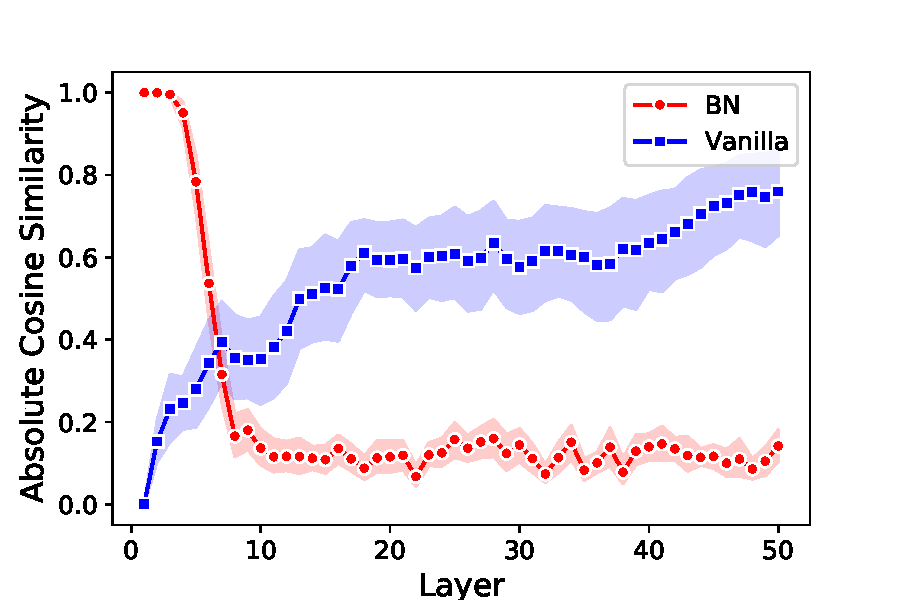
\includegraphics[width=0.4\textwidth]{figures/warmup.pdf}
    \end{tabular}
    \caption{\textbf{Orthogonality: BN vs. vanilla networks.} The horizontal axis shows the number of layers, and the vertical axis shows the absolute value of cosine similarity between two samples across the layers ($d=32$). Mean and 95\% confidence intervals of 20 independent runs.
    }
    \label{ortho:fig:orthogonality}
\end{figure}

\subsection{Theoretical analysis}
The notion of orthogonality gap plays a central role in our analysis. Given the hidden representation $H \in \R^{d\times n}$, matrix $H^\top H$ constitutes inner products between representations of different samples. Note that $H^\top H \in \R^{n \times n}$ is different form the covariance matrix $H H^\top/n \in \R^{d\times d}$. The orthogonality gap of $H$ is defined as the deviations of $H^\top H$ from identity matrix, after proper scaling. More precisely, define $V: \R^{d\times n}\setminus\mathbf{0} \to \R_+$ as 
\begin{align}
    V(H) := \Big\| \left(\frac{1}{\|H\|_F^2}\right)H^\top H - \left(\frac{1}{\|I_n\|_F^2}\right)I_n \Big\|_F.
\end{align}
% We can reformulate orthogonality gap in terms of eigenvalues of the sample covariance matrix $V(H):= \|\lambda_i/|\lambda|_1-\ones/n\|_2$, 
% where $\lambda=(\lambda_i)_{i\le n}$ are eigenvalues of $H^\top H$, and $\ones=(1)_{i\le n}$. In other words, the orthogonality gap quantifies deviations of the sample-covariance eigenvalues from their mean. For hidden representations $H_\ell$, this formula simplifies to $V(H_\ell)=\|\lambda - \ones/n\|$. Observe that $V(H)$ reaches its extreme values for perfectly orthogonal and perfectly correlated matrices $H$.  
The following theorem establishes a bound on the orthogonality of representation in layer $\ell$.
\begin{theorem} \label{ortho:thm:contraction}
Under Assumption \ref{ortho:assume:lineary_indepdence}$(\alpha,\ell)$, the following holds:
    \begin{align}\label{ortho:eq:exponential_contraction}
        \E \left[ V(H_{\ell+1}) \right] \leq 2 \left(1-\frac{2}{3}\alpha\right)^{\ell}+ \frac{3 n}{\alpha\sqrt{d}}.
    \end{align}
\end{theorem}
\noindent Assumption \ref{ortho:assume:lineary_indepdence} is studied by   \cite{daneshmand2020batch} who note that \ref{ortho:assume:lineary_indepdence}$(\alpha,\infty)$ holds as long as $d=\Omega(n^2)$. If \ref{ortho:assume:lineary_indepdence} does not hold, one can still prove that there is a function of representations that decays with depth up to a constant (see Section~\ref{ortho:sec:proof_thm}).


The above result implies that BN is an approximation algorithm for orthogonalizing the hidden representations. If we replace $\diag(M)^{-1}$  by $(M)^{-1}$ in BN formula, in Eq.~\eqref{ortho:eq:chain_linear}, then all the hidden representation will become exactly orthogonal.  However, computing the inverse of a \textit{non-diagonal} $d\times d$ matrix is computationally expensive, which must repeat for all layers throughout training, and differentiation must propagate back through this inversion. The diagonal approximation in BN significantly reduces the computational complexity of the matrix inversion. Since the orthogonality gap decays at an exponential rate with depth, the approximate orthogonality is met after only a few layers. Interestingly, this yields a desirable cost-accuracy trade-off: For a larger width, the orthogonality is more accurate, due to term $1/\sqrt{d}$ in the orthogonality gap, and also the computational gain is more significant.   



From a different angle, Theorem~\ref{ortho:thm:contraction} proves the stochastic stability of the Markov chain of hidden representations. In expectation, stochastic processes may obey an inherent Lyapunov-type of stability  \citep{kushner1967stochastic,kushner2003stochastic,khasminskii2011stochastic}. One can analyze the mixing and hitting times of Markov chains based on the stochastic stability of Markov chains,\citep{kemeny1976markov,eberle2009markov}.  
In our analysis, the orthogonality gap is a Lyapunov function characterizing the stability of the chain of hidden representations. This stability opens the door to more theoretical analysis of this chain, such as studying mixing and hitting times. For, example the stability can be used for mixing analysis of the chain $\{H_1, \dots, H_\ell,\dots \}$. Let $\pi$ denote the stationary distribution of this chain. Under a particular stochastic stability condition called geometric drift condition, 
 \begin{align*}
      \left| \E \left[ \varphi(H_\ell) \right] - \E_{H \sim \pi} \left[ \varphi(H) \right] \right| \leq \alpha^{\ell} \left| \E \left[ \varphi(H_0) \right] - \E_{H \sim \pi} \left[ \varphi(H) \right] \right|
 \end{align*}
 holds for $\alpha \in (0,1)$ and measurable function $\varphi: R^{d\times n} \to R$  (see Theorem 3.6  of \citep{hairer2010convergence}). The drift condition holds if there exists a Lyapunov function $L: R^{d\times n} \to [0,1]$ and constant $K\geq 0$ such that the following holds: 
 \begin{align*}
     E \left[ L(H_{\ell+1})| H_\ell \right] \leq \gamma L(H_{\ell}) + K. 
 \end{align*}
 We prove that the above condition holds in Eq~\eqref{ortho:eq:lyp_condition}. However, such theoretical analyses may not be of interest to the machine learning community, hence we focus on the implications of these results for understanding the underpinnings of neural networks.


It is helpful to compare the orthogonality gap in BN networks to studies on vanilla networks \citep{bjorck2018understanding,daneshmand2020batch,saxe2013exact}. The function implemented by a vanilla linear network is a linear transformation as the product of random weight matrices. The spectral properties of the product of i.i.d.~random matrices are the subject of extensive studies in probability theory~\citep{bougerol2012products}. Invoking these results, one can check that the orthogonality gap of the hidden representations in vanilla networks rapidly increases since the rank of representations converges to a one matrix as the depth grows~\citep{daneshmand2020batch}. 
% We refer readers to Section~\ref{ortho:sec:vanilla_theory} for more details about vanilla networks. 

Remarkably, \cite{agarwal2021deep} proves if activation functions obey a self-normalization property, then a specific kernel of hidden representations becomes well-condition as the network depth grows. However, it is not clear how to impose the self-normalization property. Here, we establish the whitening for an explicitly defined normalization used in practice. 



\subsection{Experimental validations}
Our experiments presented in Fig.~\ref{ortho:fig:spectral_contraction_1} validate the  exponential decay rate of $V$ with depth. In this plot, we see that $\log(V_\ell)$ linearly decreases for $\ell=1, \dots, 20$, then it wiggles around a small constant.  Our experiments in Fig.~\ref{ortho:fig:spectral_contraction_2} suggest that the $\bigo(1/\sqrt{d})$ dependency on width is  almost tight. Since $V(H_\ell)$ rapidly converges to a ball, the average of $V(H_\ell)$ over layers estimates the radius of this ball. This plot shows how the average of $V(H_\ell)$, over 500 layers, changes with the network width, validating the $\bigo(1/\sqrt{d})$ dependency implied by Theorem~\ref{ortho:thm:contraction}. 
 \begin{figure}[!ht]
     \centering
     \begin{subfigure}[b]{0.4\textwidth}
         \centering
         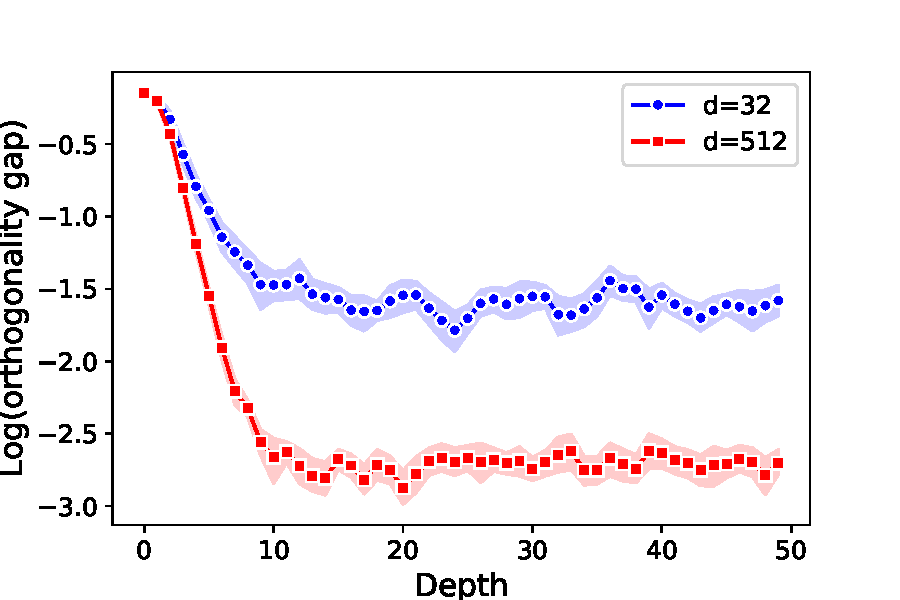
\includegraphics[width=\textwidth]{figures/gaps_depth_bn.pdf}
         \caption{Orthogonality vs. depth}
         \label{ortho:fig:spectral_contraction_1}
     \end{subfigure}
     \begin{subfigure}[b]{0.4\textwidth}
         \centering
         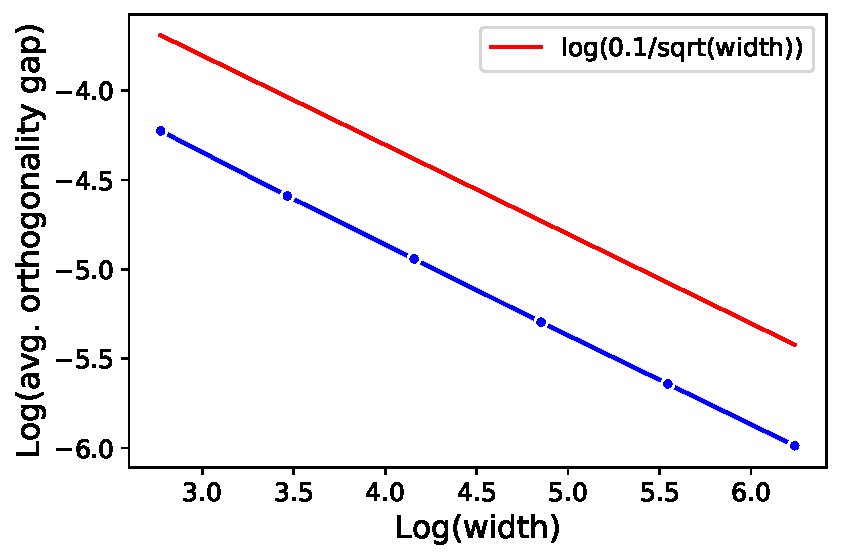
\includegraphics[width=\textwidth]{figures/gaps_width_bn.pdf}
         \caption{Orthogonality vs. width}
         \label{ortho:fig:spectral_contraction_2}
     \end{subfigure}
    \caption{\footnotesize{\textbf{Orthogonality gap vs.\ depth and width.} Left: $\log(V(H_\ell))$ vertically versus $\ell$ horizontally. Right: $\log(\frac{1}{500}\sum_{\ell=100}^{600} V(H_\ell))$ vertically versus $\log(d)$ horizontally. The chain starts from a diagonal $H_0$ with one relatively large diagonal value. This structure imposes a large orthogonality gap for $H_0$.  Mean and 95\% confidence interval of 20 independent runs.}  }
        % \label{ortho:fig:spectral_contraction}
\end{figure}

Consider an input matrix $H_0 \in \R^{d\times n}$ containing $n$ samples in $\R^d$. Assuming that elements of this matrix are i.i.d. zero-mean and unit variance random variables, the minimum singular value of $H_0$ is greater than $\sqrt{d}-\sqrt{n}$. In practical applications, the batchsize used for normalization is relatively smaller than the network width, hence  \ref{ortho:assume:lineary_indepdence}$(\Theta(1),0)$ holds. For the intermediate representations,  we also observed that  \ref{ortho:assume:lineary_indepdence}($\alpha$,$\ell$) holds --for an $\alpha$ independent from $\ell$-- as long as $d \gg n$. Let $\alpha_0$ denote the minimum singular value of $H_0$. For different values of $d$ and $n$, we check whether \ref{ortho:assume:lineary_indepdence}($0.1\alpha_0$, $1000$) holds. Fig.~\ref{ortho:fig:assumption_nd} illustrates that this assumption hold for $d= \Omega(n^2)$, which is also confirmed by \cite{daneshmand2020batch}.



\begin{figure}[!ht]
     \centering
         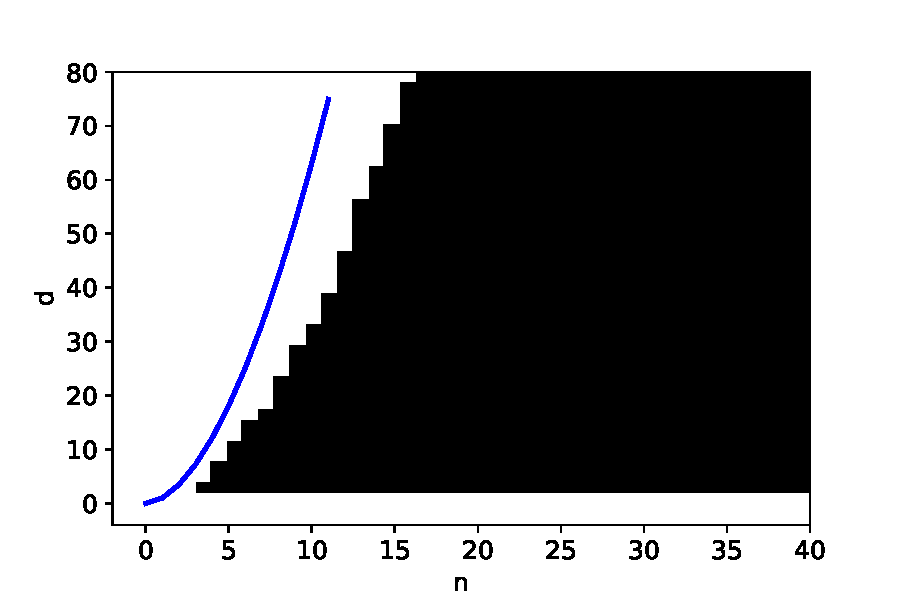
\includegraphics[width=0.5\textwidth]{figures/assumption_nd.pdf}
    \caption{\footnotesize{\textbf{Validations for \ref{ortho:assume:lineary_indepdence}} Pixel $(n,d)$ marks whether \ref{ortho:assume:lineary_indepdence} holds in all 10 independent runs: The black color indicates \ref{ortho:assume:lineary_indepdence}$(0.1\alpha_0,1000)$ failed in at least once (where $\alpha_0$ is the minimum singular value of $H_0$). The blue curve marks $d=(n-28)^{1.8}$ highlighting \ref{ortho:assume:lineary_indepdence} holds for $d = \Omega(n^2)$.} }
    \label{ortho:fig:assumption_nd}
\end{figure}



\section{Gaussian approximation} \label{ortho:sec:normal_approximation}
\subsection{Orthogonality yields Gaussian approximation}
The established result on the orthogonality gap allows us to show that the representations after linear layers are approximately Gaussian. If $H_\ell$ is orthogonal, the random matrix $W_\ell H_\ell$ is equal in distribution to a standard Gaussian matrix due to the invariance of standard Gaussian distribution under linear orthogonal transformations. We can formalize this notion of Gaussianity by bounding the Wasserstein-2 distance between the distribution of $W_\ell H_\ell$ and standard Gaussian distribution. Let $\mathcal{W}_2(R_1,R_2)$ denote the Wasserstein-2 distance between probability distributions of two random variables $R_1$, and $R_2$.
% Recall that $\mathcal{W}_2$ distance between laws of two random matrices $P, Q \in \R^{d \times n}$ is obtained by the infimum of couplings between these two random variables as
% \begin{align} \label{ortho:eq:w_distance}
%     \mathcal{W}_2\left(\law(P),\law(Q)\right)^2 = \inf_{\gamma \in \Gamma} \int \| P - Q \|_F^2 d\gamma(P, Q),
% \end{align}
% where $\Gamma$ is the set of all couplings between $\law(P)$ and $\law(Q)$ (see Chapter 1 of  \cite{villani2009optimal}). 
The next lemma formally establishes the link between the orthogonality and the distribution of the representations. 
\begin{lemma} \label{ortho:lemma:wv_bound}
Given $G \in \R^{d\times n}$ with i.i.d. zero-mean $1/d$-variance Gaussian elements, the following Gaussian approximation holds:
\begin{align}
\label{ortho:eq:bn_recurrence}
    \mathcal{W}_2\left( W_\ell H_\ell , 
    G/\sqrt{n}\right)^2 \leq 2 n \E \left[ V(H_\ell) \right].
\end{align}
\end{lemma}
Combining the above result with Theorem~\ref{ortho:thm:contraction} yields the result presented in the next corollary.
\begin{corollary} \label{ortho:cor:gaussian_approximation}
For $G \in \R^{d\times n}$ with i.i.d. zero-mean $1/d$-variance Gaussian elements, 
\begin{align}
    \mathcal{W}_2\left( W_\ell H_\ell, G/\sqrt{n}\right)^2 \leq 4n \left(1-\frac{2}{3}\alpha\right)^{\ell}+ \frac{6 n^2}{\alpha\sqrt{d}}
\end{align}
holds under Assumption~\ref{ortho:assume:lineary_indepdence}$(\alpha,\ell)$.
\end{corollary}

% \paragraph{Proof idea:} Let $H_\ell=U S V^\top$ denote the SVD decomposition of $H_\ell$ in the reduced form\footnote{We have $U\in \R^{d\times n}, S\in\R^{n\times n}, V\in\R^{n\times n}$}. If we ignore the scaling $S$ for the moment, if we transport distribution of of $W_\ell$ to $(W_\ell H_\ell)$ via rotation matrix $U$, followed by a second rotation $V^\top$ to $W_\ell (U V^\top)$, implying that $W_\ell U V^\top$ has zero Wasserstein-2 distance to $W_\ell$. The main idea is to couple weight matrix $W_\ell$ and $G$ according rotation matrices to upper bound the Wasserstein-2 distance. 


In other words, the distribution of the representations contracts to a Wasserstein 2 ball around an isotropic Gaussian distribution as the depth grows. The radius of the Wasserstein 2 ball is at most $\bigo(1/\sqrt{\text{width}})$.
As noted in the last section, \ref{ortho:assume:lineary_indepdence} is extensively studied by \cite{daneshmand2020batch} where it is shown that \ref{ortho:assume:lineary_indepdence}$(\alpha>0,\infty)$ holds as long as $d = \Omega(n^2)$. 

% Next, we compare this result with Gaussian approximations the literature. 
\subsection{Deep neural networks as Gaussian processes}
Leveraging BN, Corollary~\ref{ortho:cor:gaussian_approximation} establishes the first \textit{non-asymptotic} Gaussian approximation for deep random neural networks. For vanilla networks, the Gaussianity is guaranteed only in the \textit{asymptotic} regime of infinite width~\citep{garriga2018deep,neal2012bayesian,lee2017deep,neal2012bayesian,hazan2015steps}. Particularly, \cite{matthews2018gaussian} links vanilla networks to Gaussian processes when their width is infinite and grows in successive layers, while our Gaussian approximation holds for networks with finite width across layers. 
Table \ref{ortho:tab:normal} briefly compares Gaussian approximation for vanilla and BN networks.

\begin{table}[!ht]
    \centering
    \begin{tabular}{l l l l l l}
    \hline
      Network  & Width & Depth & Distribution of Outputs \\
    \hline 
     Vanilla MLP  & infinite  & finite & Converges to Gaussian as  width $\to \infty$ \\ 
    Vanilla Convnet  & infinite &
    finite & Converges to Gaussian as width $\to \infty$  \\
    BN MLP (Cor.~\ref{ortho:cor:gaussian_approximation}) &
    (in)finite & (in)finite & In a $\bigo(\text{width}^{-\sfrac{1}{4}})$-$\mathcal{W}_2$ ball around Gaussian\\
    \hline
    
\end{tabular}
    \vspace{0.07cm}
    \caption{\footnotesize{\textbf{Distribution of representations in random vanilla and BN networks.} For the convolutional network, the width refers to the number of channels. Results for Vanilla MLPs and Vanilla convolution networks are establish by \cite{matthews2018gaussian}, and \cite{garriga2018deep}, respectively. Remarkably, Corollary~\ref{ortho:cor:gaussian_approximation} holds for MLP with linear activations.}}
    \label{ortho:tab:normal}
\end{table}
The link between Gaussian processes and infinite-width neural networks has inspired several studies to rely on Gaussian representations in deep random networks \citep{klambauer2017self,de2018random,pennington2018emergence,schoenholz2016deep,yang2018a}. Assuming the representations are Gaussian,  \cite{klambauer2017self} designed novel activation functions that improve the optimization performance, \cite{de2018random} studies the sensitivity of random networks, \cite{pennington2018emergence} highlights the spectral universality in random networks, \cite{schoenholz2016deep} studies information propagating through the network layers, and \cite{yang2018a} studies gradients propagation through the depth.  Indeed, our analysis implies that including BN imposes the Gaussian representations required for these analyses. 
% Although our result is established for linear activations, we conjecture a similar result holds for non-linear MLPs  (see Section~\ref{ortho:sec:activations}). 

 
% \subsection{Experimental validation of the Gaussianity}
% Since the established bound in the Corollary~\ref{ortho:cor:gaussian_approximation} is non-asymptotic, we can empirically validate it. 
% Fig.~\ref{ortho:fig:wasserstein_decay} depicts the linear decay of the empirical Wasserstein distance (more details in Section~\ref{ortho:sec:wasserstein_est}) with depth, as it is predicted by Corollary~\ref{ortho:cor:gaussian_approximation}. Also, we see the decay is up to a constant inversely relates to the network width. 

%  \begin{figure}[!ht]
%      \centering
%      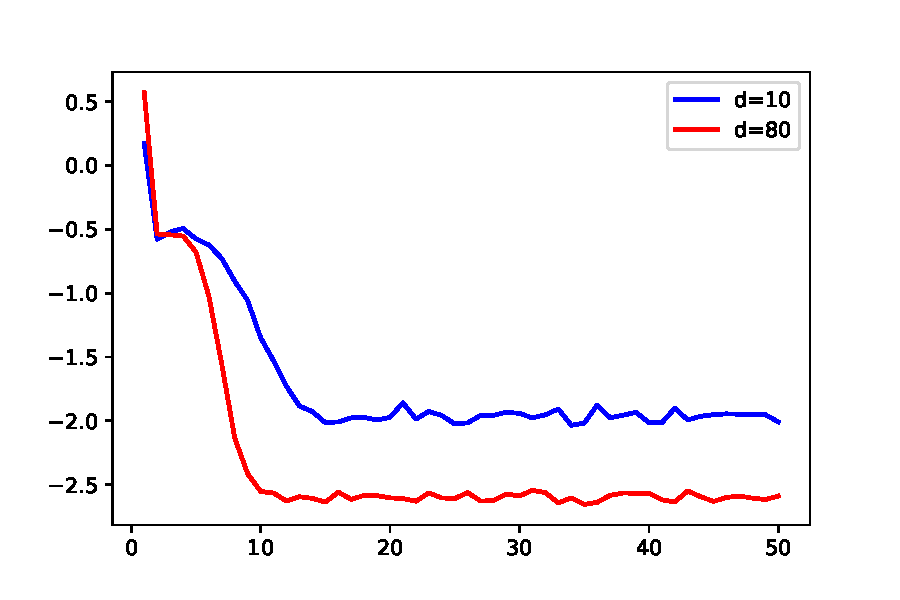
\includegraphics[width=0.45\textwidth]{figures/wdist_bn.pdf}
%      \caption{\footnotesize{\textbf{Gaussian approximation.} The empirical Wasserstein distance (vertical) between the distribution of the network outputs and Gaussian distribution, i.e.   $\log(\mathcal{W}_2(\law(W_\ell H_\ell)),\law(G/\sqrt{n})))$ width $\ell$ (horizontal). See details in Section~\ref{ortho:sec:wasserstein_est}.}}
%      \label{ortho:fig:wasserstein_decay}
%  \end{figure}

\section{The orthogonality and optimization}
\label{ortho:sec:optimization}
In the preceding sections, we elaborated on the theoretical properties of BN networks in controlled settings. 
In this section, we demonstrate the practical applications of our findings. In the first part, we focus on the relationship between depth and orthogonality. Increasing depth drastically slows the training of neural networks with BN. Furthermore, we observe that as depth grows, the training slowdown highly correlates with the orthogonality gap. This observation suggests that SGD needs to orthogonalize deep representations in order to start classification. This intuition leads us to the following question: If orthogonalization is a prerequisite for training, can we save optimization time by starting from orthogonal representations? To test this experimentally, we devised a weight initialization that guarantees orthogonality of representations. Surprisingly, even in a network without BN, our experiments showed that this initialization avoids the training slow down, affirmatively answering the question. 

Throughout the experiments, we use vanilla MLP (without BN) with a width of 800 across all hidden layers, ReLU activation, and used Xavier's method for weights intialization~\citep{glorot2010understanding}. We use SGD with stepsize $0.01$ and batch size $500$ and for training. The learning task is classification with cross entropy loss for CIFAR10 dataset~\citep[][MIT license]{krizhevsky2009learning}. We use PyTorch~\citep[][BSD license]{NEURIPS2019_9015} and Google Colaboratory platform with a single Tesla-P100 GPU with 16GB memory in all the experiments. The reported orthogonality gap is the average of the orthogonality gap of representation in the last layer.


\subsection{Orthogonality correlates with optimization performance}
In the first experiment, we show that the orthogonality of representations at the initialization correlates with optimization speed. For networks with 15, 30, 45, 60, and 75 widths, we register training loss after 30 epochs and compare it with the initial orthogonality gap. Figure~\ref{ortho:fig:slowdown_depth} shows the training loss (blue) and the initial orthogonality gap (red) as a function of depth. We observe that representations are more entangled, i.e., orthogonal, when we increase depth, coinciding with the training slowdown.  Intuitively, the slowdown is due to the additional time SGD must spend to orthogonalize the representations before classification. In the second experiment, we validate this intuitive argument by tracking the orthogonality gap during training. Figure~\ref{ortho:fig:slowdown_training} plots the orthogonality gap of output and training loss for a network with 20 layers. We observe that SGD updates are iteratively orthogonalizing representations, marked by the reduction in the orthogonality gap.

 \begin{figure}[!ht]
     \centering
     \begin{subfigure}[b]{0.4\textwidth}
         \centering
         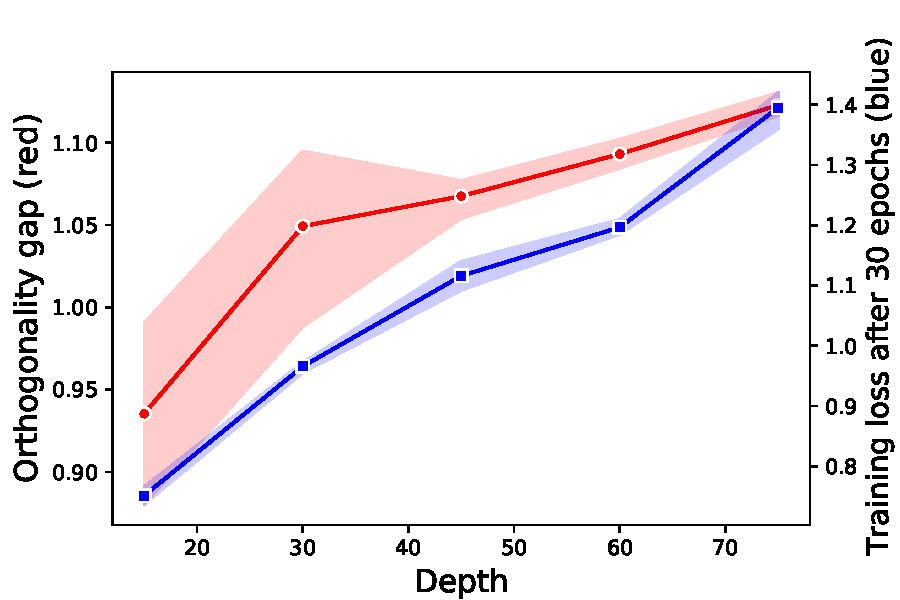
\includegraphics[width=\textwidth]{figures/gaps_loss_depth.pdf}
         \caption{gap and loss vs. depth}
         \label{ortho:fig:slowdown_depth}
     \end{subfigure}
     \begin{subfigure}[b]{0.4\textwidth}
         \centering
         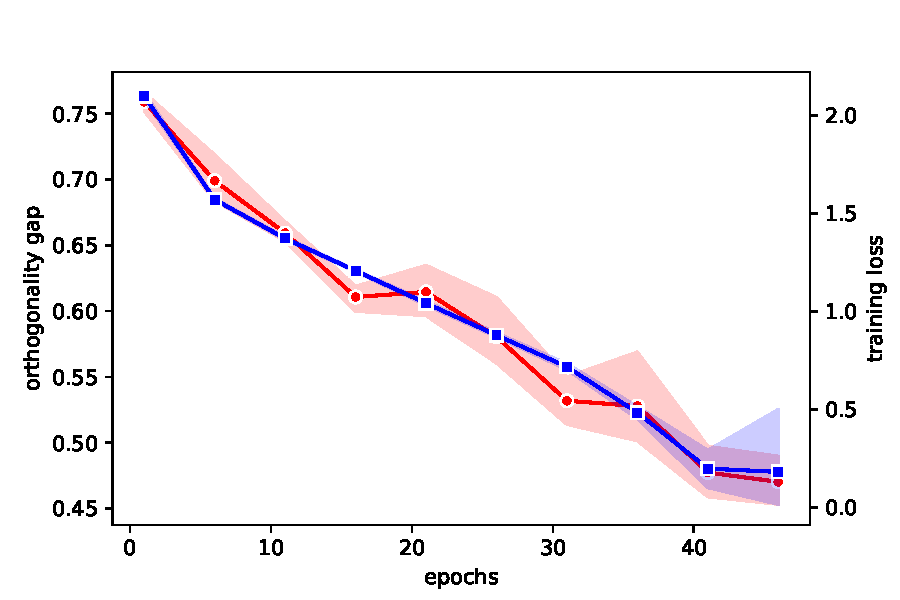
\includegraphics[width=\textwidth]{figures/gaps_training.pdf}
         \caption{gap and loss during training}
         \label{ortho:fig:slowdown_training}
     \end{subfigure}
    \caption{\footnotesize{\textbf{Orthogonality and Optimization} Left: the orthogonality gap at initialization (red, left axis) and the training loss after 30 epochs (blue, right axis) with depth. Right: the orthogonality gap (red, left axis) and  the training loss in each epoch (blue, right axis). Mean and 95\% confidence interval of 4 independent runs. }}
        \label{ortho:fig:slowdown_orthogonality}
\end{figure}


\subsection{Learning with initial orthogonal representations}
We have seen that the slowdown in SGD for deeper networks correlates with the orthogonality gap before training.
Here we show that by preemptively orthogonalizing representations, we avoid the slowdown with depth. While in MPL with linear activations, hidden representations remain orthogonal simply by taking orthogonal matrices as weights~\citep{pennington2018emergence,saxe2013exact}, the same does not hold for networks with non-linear activations, such as ReLU. To enforce the orthogonality in the absence of BN, we introduce a dependency between weights of successive layers that ensures deep representations remain orthogonal. More specifically, we incorporate the SVD decomposition of the hidden representation of each layer into the initialization of the subsequent layer. To emphasis this dependency between layers and to distinguish it from purely orthogonal weight initialization, we refer to this as \emph{iterative orthogonalization}.

We take a large batch of samples $n\geq d$, as the input batch for initialization. Let us assume that weights are initialized up to layer $W_{\ell-1}$. To initialize $W_\ell$, we  compute SVD decomposition of the representations $H_\ell = U_\ell \Sigma_\ell V^\top_\ell$ where matrices $U_\ell \in \R^{d \times d}$ and $V_\ell \in \R^{n \times d}$ are orthogonal. Given this decomposition, we initialize $W_\ell$ by 
\begin{align} \label{ortho:eq:init_w}
    W_\ell = \frac{1}{\| \Sigma_\ell^{\sfrac{1}{2}}\|_F} V_\ell' \Sigma_\ell^{-\sfrac{1}{2}} U_\ell^\top,
\end{align}
where $V'_\ell \in \R^{d\times d}$ is an orthogonal matrix obtained by slicing $V_\ell \in \R^{n\times d}$. Notably, the inverse in the above formula exists when $n$ is sufficiently larger than $d$ \footnote{We may inductively assume that $H_\ell$ is almost orthogonal by the choice of $W_1, \dots, W_{\ell-1}$. Thus, $\Sigma_\ell$ is invertible. }. 
It is easy to check that  $V(W_\ell H_\ell)< V(H_\ell)$ holds for the above initialization (see Section~\ref{ortho:sec:init}), similar to BN. 
%We observed this method effectively orthogonalizes hidden representations when the batch size is sufficiently large. Fig.~\ref{ortho:fig:cifar_orthogonal_a} compares the orthogonality gap of the representations for this initialization method with a standard initialization. 
By enforcing the orthogonality, this initialization significantly alleviates the slow down of training with depth (see Fig.~\ref{ortho:fig:cifar_orthogonal}), with no need for BN. This initialization is not limited to MLPs. In Section~\ref{ortho:sec:bnreplace}, we compare iterative orthogonalization with a BN-replacement method recently proposed by \cite{brock2021high}.  
% In Section~\ref{ortho:sec:experiments}, we propose a similar SVD-based initialization for convolutional networks that effectively accelerates the training of deep convolutional networks.  

 \begin{figure}[!ht]
     \centering
         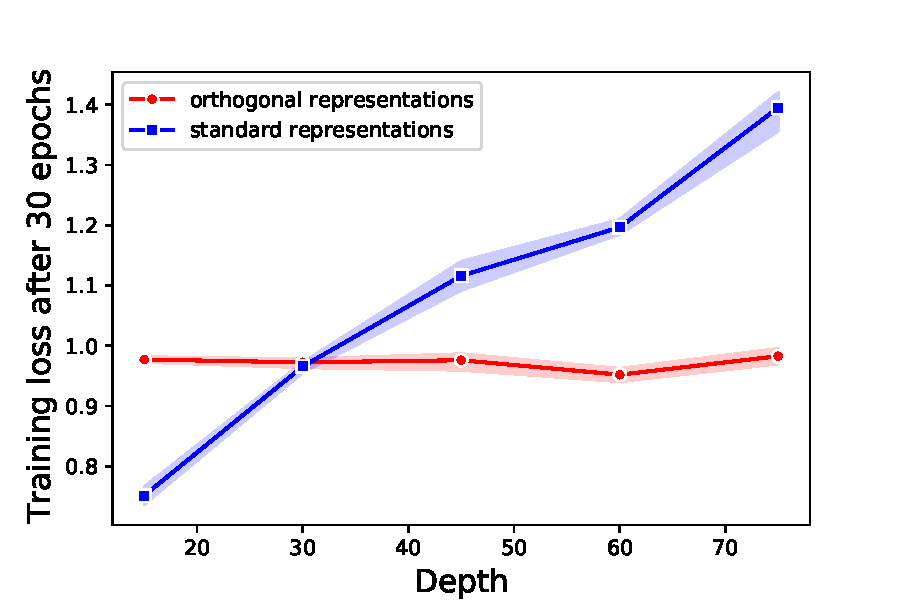
\includegraphics[width=0.55\textwidth]{figures/training_orth.pdf}
    \caption{\footnotesize{\textbf{Iterative orthogonalization.} Horizontal axis: depth. Vertical axis: the training loss after 30 epochs for Xavier's initialization (blue), our initialization (red). Mean and 95\% confidence interval of 4 independent runs.}}
        \label{ortho:fig:cifar_orthogonal}
\end{figure}



\section{Discussion}
To recap, we proved the recurrence of random linear transformations and BN orthogonalizes samples. Our experiments underline practical applications of this theoretical finding: starting from orthogonal representations effectively avoids the training slowdown with depth for MLPs. Based on our experimental observations, a proper initialization ensuring the orthogonality of hidden representations may replace BN in neural architectures. This future research direction has the potentials to boost the training of deep neural networks and change benchmarks in deep learning.


Although our theoretical bounds hold for MLPs with linear activations, our experiments confirm similar orthogonal stability for various neural architectures. 
%  Figure~\ref{ortho:fig:relu_convnet} demonstrates this stability for MLPs with ReLU activations and a convolutional networks. This plot compares the evolution of the orthogonality gap, through layers, for BN networks with vanilla networks. For vanilla networks, we observe that the gap increases with depth. On the contrary, the gap decreases by adding BN layers and stabilizes at a term that is constant with regard to depth. Based on our observations, we conjecture that hidden representations of modern BN networks obey similar stability. A more formal statement of the conjecture is presented in Section~\ref{ortho:sec:activations}. 

\cite{lubana2021beyond} experimentally compares properties of different normalization techniques including layer normalization (LN)~\citep{ba2016layer}. According to this study,  LN does not necessarily orthogonalize the outputs of deep neural networks. Hence, more theoretical studies are required to understand the essence of different normalization techniques in deep learning.
% \section*{Acknowledgements}
%  We thank Gideon Dresdner, Vincent Fortuin, and Ragnar Groot Koerkamp for their helpful comments and discussions. This work was funded in part by the French government under management of Agence Nationale de la Recherche as part of the “Investissements d’avenir” program, reference ANR-19-P3IA-0001(PRAIRIE 3IA Institute). We also acknowledge support from the European Research Council (grant SEQUOIA 724063). 


% \end{document}
